In this work, we explore the deployment of advanced reactors in the future
energy landscape of the \gls{usa}. As the landscape evolves, compounding
factors will drive the actual deployment of these reactors in ways this work
does not capture. The value of energy system modeling and this type of
transition scenario is to understand the implications of deployment compared
with and measured relatively to business-as-usual cases with similar
approximations.

We use this chapter to explore the deployment schemes we have
implemented---outlined in Table \ref{tab:deployment_schemes}---, and the demand
growth scenarios we have considered---outlined in Table
\ref{tab:demand_scenarios}. In Appendix \ref{sec:considered_deployment_schemes}
we will also discuss two additional deployment schemes that we implemented, but
not incorporated as they are more useful for problems not considered herein.

\begin{table}[htbp]
    \centering
    \caption{Deployment Schemes}
    \label{tab:deployment_schemes}
    \begin{tabular}{p{0.15\linewidth} p{0.27\linewidth} p{0.50\linewidth}}
        \hline
        \textbf{Status} & \textbf{Scheme} & \textbf{Description} \\
        \hline
        \multirow{3}{*}{Incorporated} & Greedy Deployment & Deploy the largest
        reactor first at each time step, fill in the remaining capacity with
        the next smallest, and so on. \\
        & Random Deployment & Uses a date and hour as seed to sample the
        reactors list randomly. \\
        & Initially Random, Greedy Deployment & Randomly deploys reactors until
        a reactor bigger than the remaining capacity is proposed for each year,
        then fills the remaining capacity with a greedy algorithm. \\
        \hline
        \multirow{2}{*}{Not Incorporated} & Capped Deployment & There is a
        single-number capacity for one or more of the reactor models. \\
        & Pre-Determined Distribution Deployment & One or more reactors have a
        preset distribution, and a smaller capacity model fills in the gaps. \\
        \hline
    \end{tabular}
\end{table}

We apply these deployment schemes to demand growth scenarios based on two
predictions. The \gls{eia} publishes demand expansion projections for the
totality of \gls{usa} \cite{eia_aeo_2023}. As we have discussed, the
administration has refrained from publishing AEO 2024 in light of recent
accelerations in demand growth. Our assumptions for the low-growth scenarios
are that the relative percentage of nuclear power remains constant and that the
relative performance of the various fuel cycle metrics we simulate will hold.
The \gls{doe} Liftoff Report \cite{julie_liftoff_pathways_2024} does not
reflect this constant percentage assumption for nuclear power in their demand
scenarios, which are specific to nuclear deployment increases and the number is
agnostic to the total increase.

\begin{table}[htbp]
    \centering
    \caption{Demand Growth Scenarios}
    \label{tab:demand_scenarios}
    \begin{tabular}{c c c}
        \hline
        \textbf{Demand Growth} & \textbf{Year-to-Year Increase} & \textbf{Source}\\
        \hline
 No growth & 0\% & na\\
 Low growth & 0.17\%, 0.5\%, 1\%, & \cite{eia_aeo_2023}\\
 High growth & 3.5\%, 5.6\% & \cite{julie_liftoff_pathways_2024}\\
        \hline
    \end{tabular}
\end{table}

\section{Greedy Deployment}
\label{sec:greedy_deployment}

In this scheme, we deploy the largest reactor first until another
deployment of that reactor exceeds the demand---as outlined in
\ref{fig:greedy_diagram}. Then we move to the next largest reactor until the
next deployment of the smallest capacity reactor exceeds the
demand. This scheme is not a proxy for strategic decisions by individual
actors it merely meets the demand in a roughly efficient manner.

Previous work from Bachmann et \textit{al.} \cite{bachmann_enrichment_2021}
employed a similar deployment scheme to explore the deployment of advanced
reactors in the \gls{usa}. This scheme is computationally efficient and allows
for the exploration of the deployment of advanced reactors in a way that is not
overly complex. This scheme is most useful for scenarios where the user is
interested in comparing metrics relative to the number of specific reactors
deployed outside of the context of the problem.

\begin{figure}[!htbp]
    \centering
    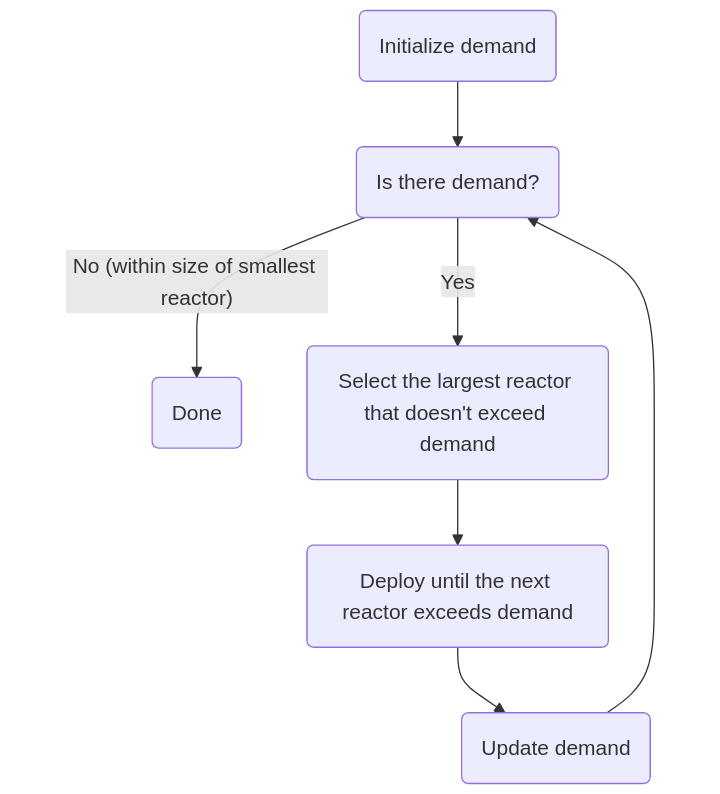
\includegraphics[scale=0.4]{images/schemes/greedy_diagram.png}
    \caption{Greedy Deployment Diagram}
    \label{fig:greedy_diagram}
\end{figure}

Through the greedy deployment, we are not attempting to capture the complexity
of the deployment problem but rather to explore the implications of deploying a
certain number of reactors. As such, we limit the discussion of realism to the
extent that the scheme meets the demand and could mirror large actors in a
market. The scheme will deploy reactors until the demand is met within the
amount of the smallest capacity reactor.



\section{Random Deployment}
\label{sec:random_deployment}

Advanced reactor concepts, like the ones outlined in this work, are often
designed for use cases ranging from industrial steam production to microgrid
integration. Our deployment of these reactors is
a complex problem that requires a nuanced understanding of the energy market,
the regulatory environment, the intended use of the technology, and the
technical capabilities of the reactor.

This random deployment is a proxy for the complexity of the real-world
deployment problem but does not include the nuance of how individual
deployments meet an end user's needs, which will drive the strategic decisions
that utilities and ratepayers behind the meter make in their reactor choices
The random deployment scheme has the potential to capture some of the
complexities in overall market development, but the extent we capture these
details is not explored in this work.

The random deployment scheme is implemented by randomly selecting reactors from
the list of deployable reactors until the demand is covered. We illustrate this
scheme in Figure \ref{fig:random_diagram}, which shows the single loop in the
logic from the top down. There is an irreducible demand that cannot be met
because the power capacity is assumed to be constant. As such the random
deployment scheme, at its best, will meet the demand, but has the potential to
fall short of the demand by one of the smallest capacity reactors. To reduce
the computational cost of this scheme, we have implemented a rough random case
that deploys until the randomly selected reactor exceeds the demand. This rough
approximation is what we couple with the greedy deployment scheme in the
initially random, greedy deployment scheme in Section
\ref{sec:initially_random_greedy}.

\begin{figure}[!htbp]
    \centering
    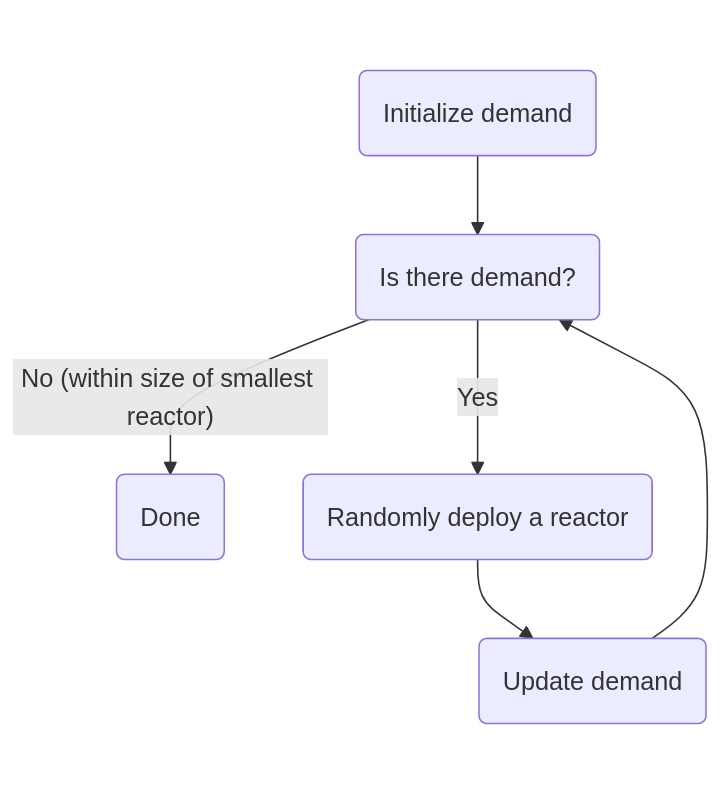
\includegraphics[scale=0.4]{images/schemes/random_diagram.png}
    \caption{Random Deployment Diagram}
    \label{fig:random_diagram}
\end{figure}

The seed for the random number generator is set by the date and time of the
simulation, which allows for the reproducibility of the results. This scheme is
a proxy for aggregate decisions by actors and would fail to reliably capture
individual actor decisions. This scheme is most useful for scenarios or
timescales where there is a high degree of uncertainty in the deployment of
reactors.


\section{Initially Random, Greedy Deployment}
\label{sec:initially_random_greedy}

Combining the random and greedy deployment schemes allows us to inject some of
the uncertainty around which reactor will be deployed at any given time while
ensuring that the demand is met in a reasonably computationally efficient
manner. This scheme does not give us more insight than the random or greedy
deployment schemes it merely allows us to leverage the strengths of both.

In this deployment scheme, we randomly deploy reactors until a reactor bigger
than the remaining capacity is proposed for each year, then fill the remaining
capacity with a greedy algorithm. We outline this scheme in Figure
\ref{fig:init_random_greedy_diagram}, which shows the two loops (first random,
then greedy) in the logic from the top down.

\begin{figure}[!htbp]
    \centering
    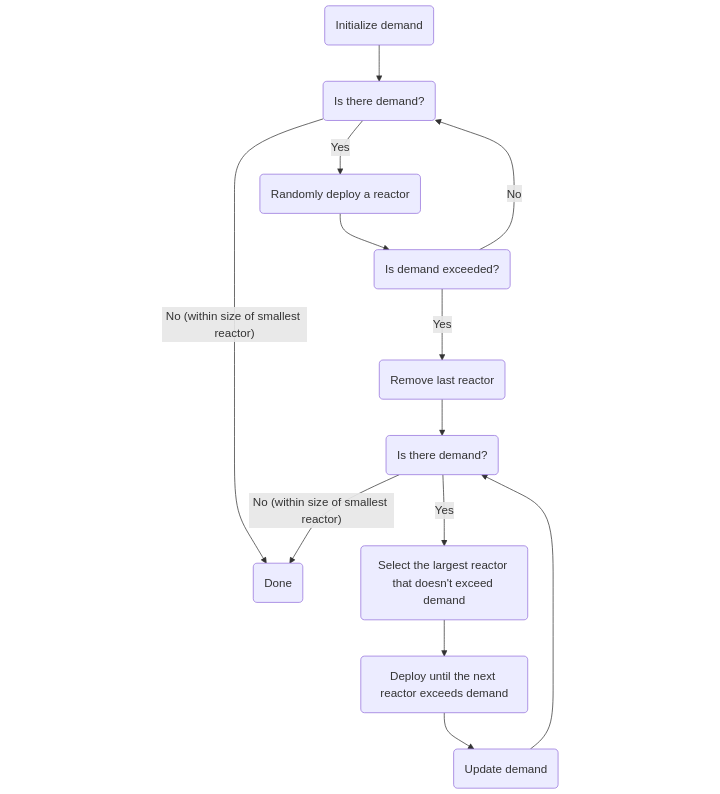
\includegraphics[scale=0.7]{images/schemes/random_greedy_diagram.png}
    \caption{Initially Random, Greedy Deployment Diagram}
    \label{fig:init_random_greedy_diagram}
\end{figure}

As highlighted in Section \ref{sec:random_deployment}, we did not implement the
initially random, greedy deployment scheme to capture additional realism in the
deployment problem. This scheme combines random and greedy deployment schemes
and inherits their realistic and unrealistic elements. The random deployment
scheme captures some of the complexity of the deployment problem but does not
guarantee the capture of the nuance of future user needs. The greedy deployment
scheme captures the efficiency of the deployment problem but does not capture
the complexity of the deployment problem. This scheme is a compromise between
the two and does not capture the nuance of the deployment problem.

The degree to which this scheme captures features of the random or greedy
deployment schemes varies with the number of reactors deployed in the random
phase. Instead of randomly deploying until the demand is met, this
implementation randomly deploys until the selected reactor exceeds the demand.
This means that when the reactors are different sizes, there is a chance that
the random phase will deploy a reactor that is much larger than the demand, and
the greedy phase will make up more of the deployment.